\section{ROS - First Steps}

\begin{frame}
	\frametitle{O que é o ROS?}

	\only<1>
	{
		\begin{itemize}
			\item ROS é um \textit{framework open source} para o desenvolvimento de software para robôs
			\item Provê uma funcionalidade análoga a de um sistema operacional
		\end{itemize}
	}

	\only<2>
	{
		\begin{itemize}
			\item Provês serviços de sistema operacional
			\item Abstração de hardware
			\item Controle de dispositivos em baixo nível
			\item Implementação de funcionalidades comumente utilizadas 
			\item Transferência de mensagens entre processos
			\item Gerenciamento de pacotes
		\end{itemize}
	}
	\only<3>
	{
		\centering
		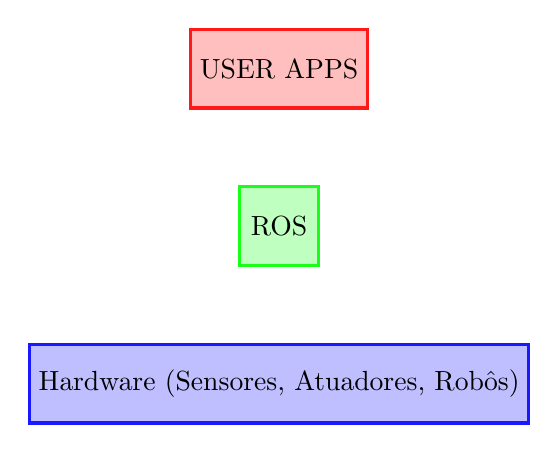
\begin{tikzpicture}
			[vermelho/.style={rectangle, draw=red!90, 	fill=red!25, 	very thick, minimum size = 10mm},
			verde/.style	={rectangle, draw=green!90, fill=green!25, 	very thick, minimum size = 10mm},
			azul/.style		={rectangle, draw=blue!90, 	fill=blue!25, 	very thick, minimum size = 10mm},]			
			\node[vermelho] 						(aps)	{USER APPS};
			\node[verde,below of=aps ,yshift=-1cm]	(ros) 	{ROS};
			\node[azul, below of=ros ,yshift=-1cm] 	(ser)	{Hardware (Sensores, Atuadores, Robôs)};
		\end{tikzpicture}			
	}
\end{frame}

\begin{frame}
	\frametitle{Ecossistema ROS} 
	\only<1>
	{
		\centering
		\includegraphics[width=9cm,height=6cm]{Figuras/RosEcosystem.png} \\~\\
		\footnote{\scriptsize ROS Robot Programming (in English).Authors:Yoonseok Pyo, Hancheol Cho, Leon Jung, Darby Lim}
	}
	\only<2>
	{
		\centering
		\includegraphics[width=11cm,height=6cm]{Figuras/universoROS.png} 
	}	
\end{frame}

\begin{frame}
	\frametitle{Por que usar ROS?}
	\begin{itemize}
		\item Re-utilização de códigos em Robótica (P\&D)
		\item Ambiente de desenvolvimento pronto para utilizar
		\item Contínuo suporte 
		\item Ferramentas amigáveis
		\item Concebido para ser escalável
		\item Comunidade ativa ao redor do mundo. \scriptsize Clique em: \href{http://answers.ros.org}{\underline{http://answers.ros.org}}
	\end{itemize}
	\centering
	\includegraphics[width=2cm,height=1cm]{Figuras/ROSAnswers.png} 
\end{frame}

\begin{frame}
	\frametitle{Configurando o Ambiente de Trabalho - Sistemas Operacionais}
	\centering
	\includegraphics[width=7.5cm,height=6cm]{Figuras/SistemasOperacionais.png}
	\begin{itemize}
		\item Pode ser utilizado em conjunto com a maioria dos sistemas operacionais
		\item É recomendado o Ubuntu como sistema operacional mais estável
	\end{itemize}

\end{frame}

\begin{frame}
	\frametitle{Ambiente de Desenvolvimento}
	\begin{itemize}
		\item \underline{\textbf{Hardware}}: \textit{Desktop} ou \textit{laptop} usando processador Intel ou AMD
		\item \underline{\textbf{Sistema Operacional}}: Ubuntu (versão compatível com a versão do ROS - verificar site oficial
		\item \underline{\textbf{ROS}}: Noetic Ninjemys
	\end{itemize}
\end{frame}

\begin{frame}
	\frametitle{Máquinas Virtuais}
	\begin{table}
		\begin{tabular}{  >{\centering\arraybackslash}m{1cm}  >{\centering\arraybackslash}m{7cm}  }  
			\includegraphics[width=1cm,height=1cm]{Figuras/VirtualBox.png} & Virtual Box (\href{www.virtualbox.org}{\underline{www.virtualbox.org}})\\
			\includegraphics[width=1.4cm,height=1cm]{Figuras/Parallels.png} & Parallels (\href{www.parallels.com}{\underline{www.parallels.com}}) \\
			\includegraphics[width=1cm,height=1cm]{Figuras/VMWare.png} & VMWare (\href{www.vmware.com}{\underline{www.vmware.com}})\\
		\end{tabular}
	\end{table}
	
	\centering
	\scriptsize
	\color{red}
	Diversas imagens de instalação do ROS disponíveis on-line
\end{frame}


\begin{frame}
    \frametitle{Preparando o Ubunto antes de Instalar o ROS}
	\only<1>
		{
		\frametitle{Instalação Geral - NTP (Network Time Protocol}
		\textit{\underline{Objetivo}}: Reduzir diferença de tempo entre os pacotes ROS na comunicação entre múltiplos computadores, ou seja, melhorar a sincronia entre os processos.
		\vspace{0.5cm}
		\begin{figure}
			\includegraphics[width=11cm,height=1.7cm]{Figuras/Ntp.png}
		\end{figure}
	}

	\only<2>
	{
		\frametitle{Instalação Geral - Adding Source List}
		\textit{\underline{Objetivo}}: Adicionar o endereço do repositório do ROS no \textit{ros.latest.list}. Abra um novo terminal e digite o seguinte comando.
		\vspace{0.5cm}
		\begin{figure}
			\includegraphics[width=11cm,height=1.7cm]{Figuras/SourceList.png}
		\end{figure}
	}

	\only<3>
	{
		\frametitle{Instalação Geral - Definindo Chave Pública}
		\textit{\underline{Objetivo}}: Define uma chave pública para acessar o repositório do ROS para o download de pacotes. Acessar a página oficial (Wiki) do ROS para atualizar a chave que pode ser alterada.
		\vspace{0.5cm}
		\begin{figure}
			\includegraphics[width=11cm,height=1.7cm]{Figuras/Chave.png}
		\end{figure}
	}

	\only<4>
	{
		\frametitle{Instalação Geral - Adding Atualizando o Sistema}
		\textit{\underline{Objetivo}}: Após a adição do endereço do repositório do ROS na lista de fontes, deve ser realizada uma nova indexação da lista de pacotes. Embora não seja mandatório, é recomendável a realização de um upgrade em todos os pacotes previamente instalados no UBUNTU antes da instalação do ROS.
		\vspace{0.5cm}
		\begin{figure}
			\includegraphics[width=11cm,height=1cm]{Figuras/Update.png}
		\end{figure}
	}

	\only<5>
	{
		\frametitle{Instalação Geral - Instalando o ROS}
		\textit{\underline{Objetivo}}: Finalmente, devemos instalar os pacotes do ROS para desktop usando o seguinte comando. Esta instalação incluirá as principais funcionalidades do ROS (ROS, rqt, RViz, robot-related-libraries, simulation, navigation, etc)
		\vspace{0.5cm}
		\begin{figure}
			\includegraphics[width=11cm,height=1cm]{Figuras/Install.png}
		\end{figure}
	}
\end{frame}

\begin{frame}
	\frametitle{Conceitos Básicos: Nó (\textit{Node})}
	\begin{itemize}
		\item O princípio básico de operação do ROS é a facilidade de modularização de processos que são executados em conjunto pelo sistema operacional
		\item Nó (ou Node): um processo que usa o framework do ROS
		\item Os nós podem ser executados em máquinas diferentes de forma transparente
		\item O \textbf{roscore} é um processo único (ou nó principal e obrigatório) que gerencia a comunicação entre todos os nós
	\end{itemize}
\end{frame}

\begin{frame}
	\frametitle{Conceitos Básicos: \textit{roscore}}
	\begin{itemize}
		\item Funciona basicamente como um name server
		\item Os nós se comunicam com o ROSCORE o qual é definido por uma variável de ambiente denominada ROS\_MASTER\_URI
	\end{itemize}
	\centering
	\includegraphics[width=8cm,height=3cm]{Figuras/roscore.png}
\end{frame}

\begin{frame}
	\frametitle{Conceitos Básicos: Tópicos}
	\begin{itemize}
		\item Tópico é o meio através do qual uma mensagem pode ser enviada de um nó para outro (ou vários outros) 
		\item A forma de comunicação segue um modelo de \textit{publisher-subscriber}
		\item \underline{\textit{Publish}}: Envia uma mensagem para um tópico
		\item \underline{\textit{Subscribe}}: São chamados caso uma mensagem é publicada
		\item As mensagens publicadas são transmitidas para todos os \textit{subscribers} 
	\end{itemize}
	\centering
	\centering
	\includegraphics[width=8.5cm,height=2.3cm]{Figuras/topicos.png}	
\end{frame}

\begin{frame}
	\frametitle{Conceitos Básicos: Serviços}
	\begin{itemize}
		\item \textit{SERVICE} é um mecanismo pelo qual um nó envia uma requisição para outro e recebe uma resposta à chamada
		\item A forma de comunicação segue um modelo \textit{request-response}
		\item Um serviço é chamado com uma estrutura de \textit{request} e, em resposta, uma estrutura de resposta é retornada
	\end{itemize}
	\centering
	\centering
	\includegraphics[width=8.5cm,height=2.3cm]{Figuras/servico.png}	
\end{frame}

\begin{frame}
	\frametitle{Conceitos Básicos: \textit{Action}}
	\begin{itemize}
		\item \textit{ACTION} é usada quando uma requisição leva longo tempo para ser executada e é necessário que a sua evolução deve ser acompanhada.
		\item É muito similar ao serviço, onde \textit{'goals'} e \textit{'results'} são análogos aos \textit{'requests'} e \textit{'responses'} do \textit{SERVICE}.
		\item Diferentemente do \textit{SERVICE}, uma \textit{ACTION} é frequentemente usado quando é necessário enviar tarefas mais complexas para o robô como, por exemplo, cancelar um objetivo previamente enviado enquanto as tarefas estão em andamento.
	\end{itemize}
	\centering
	\centering
	\includegraphics[width=6.5cm,height=2.5cm]{Figuras/Action.png}	
\end{frame}

\begin{frame}
	\frametitle{Tópicos, Serviços e Actions}
	\begin{table}
		\scriptsize
		\begin{tabular}{c c c p{4cm}}
			\hline
			\hline
			\textbf{Tipo} & \textbf{Característica} & & \textbf{Descrição} \\		
			\hline		
			Tópico			& Assíncrona	& Unidirecional & Usado quando os dados são trocados continuamente. \\
			Serviço			& Síncrona 		& Bidirecional  & Usado quando o cliente requisita e recebe um estado corrente. \\
			\textit{Action}	& Assíncrona	& Bidirecional  & Usado quando é difícil usar o serviço devido a longos tempos de resposta após a solicitação ou quando é necessário um valor de \textit{feedback} intermediário. \\
			\hline
			\hline
		\end{tabular}
	\end{table}
\end{frame}